\documentclass[11pt]{article}
\usepackage[margin=1in]{geometry}
\usepackage[utf8]{inputenc}
\usepackage[T1]{fontenc}
\usepackage{hyperref}
\usepackage{url}
\usepackage{booktabs}
\usepackage{amsfonts}
\usepackage{nicefrac}
\usepackage{microtype}
\usepackage{amsmath,amssymb}
\usepackage{graphicx}
\usepackage{multirow}
\usepackage{subcaption}
\usepackage{xcolor}
\usepackage{natbib}
\usepackage{amsthm}
\bibliographystyle{unsrtnat}

\theoremstyle{definition}
\newtheorem{definition}{Definition}[section]

\title{The Shape of Wisdom: Structured Decision Formation and \
Commitment Dynamics in Large Language Models}

\author{%
  Shailesh Rana\\
  Independent Research\\
  \texttt{shailesh.rana@gmail.com}\\
}

\begin{document}

\maketitle

\begin{abstract}
\textbf{Background:} Large language models (LLMs) exhibit remarkable reasoning capabilities, yet the internal mechanisms of how they form and commit to decisions remain poorly understood. Understanding the geometry of decision formation is critical for improving reliability and interpreting model behavior.

\textbf{Methods:} We analyzed three 7--8B parameter instruction-tuned models (Qwen2.5-7B, Llama-3.1-8B, Mistral-7B-v0.3) on 3,000 multiple-choice questions spanning eight knowledge domains. Using layer-wise hidden state analysis at the first decoding step, we measured convergence dynamics, commitment timing, and representational topology through option-token invariant scoring. We defined convergence based on probability thresholds and margin stability, and characterized commitment through winner stability across layers.

\textbf{Results:} Models exhibited substantial variation in accuracy (Qwen: 67.3\%, Llama: 60.7\%, Mistral: 54.2\%) and high-confidence convergence rates (Qwen: 46.5\%, Llama: 34.6\%, Mistral: 43.5\%). Stable commitment was detected in 40.5--53.2\% of prompts, with late-flip rates of 12.2--21.6\%. Cross-model analysis identified 904 ``universally hard'' prompts non-converged across all models. Early-layer features predicted final failure with ROC-AUC 0.65--0.71. Representational topology revealed domain-clustered structure and wrong-answer basins, with highest trajectory divergence in late-middle layers.

\textbf{Conclusion:} LLMs exhibit structured, layer-wise decision formation with measurable commitment dynamics. The predictability of failures from early layers and the existence of cross-model hard prompts suggest fundamental reasoning limitations that persist across architectures. These findings provide a mechanistic foundation for targeted interventions to improve model reliability.
\end{abstract}

\section{Introduction}

Large language models (LLMs) have demonstrated impressive performance on reasoning benchmarks, yet their internal decision-making processes remain largely opaque \citep{berglund2023reversal,meng2022locating}. While endpoint accuracy provides a coarse measure of capability, it reveals little about \textit{how} models arrive at their answers---whether through structured reasoning, spurious correlations, or stochastic sampling \citep{mccoy2019right,ribeiro2020beyond}.

This work investigates the \textbf{shape of wisdom}: the geometry and dynamics of decision formation in transformer-based language models. We ask: Do models exhibit structured commitment to answers as computation progresses through layers? Can we predict failures from early computation? Are there questions that fundamentally challenge models across architectures?

Understanding these dynamics has practical importance. If models commit to wrong answers early, interventions should target early layers. If commitment is unstable (late flips), stabilization mechanisms may help. If certain prompts universally challenge models, they may reveal fundamental knowledge gaps or reasoning limitations.

\subsection{The Commitment Hypothesis}

We hypothesize that LLMs exhibit \textit{structured decision formation} characterized by:
\begin{enumerate}
    \item \textbf{Progressive convergence}: Option probabilities become increasingly concentrated across layers
    \item \textbf{Commitment events}: Layers where the eventual winner stabilizes with sufficient margin
    \item \textbf{Predictable failures}: Early-layer signals correlate with final correctness
\end{enumerate}

This contrasts with views of models as ``stochastic parrots'' \citep{bender2021dangers} or purely pattern-matching systems. If commitment dynamics exist, they suggest models engage in something akin to ``thinking through'' answers, with computation playing a causal role in decision quality.

\subsection{Contributions}

Our contributions are:
\begin{itemize}
    \item A framework for analyzing layer-wise decision convergence using option-token invariant scoring
    \item Characterization of commitment dynamics across three major open-weight models
    \item Identification of 904 universally hard prompts that resist convergence across architectures
    \item Demonstration that early-layer features predict final failures (ROC-AUC 0.65--0.71)
    \item Topological analysis revealing domain-clustered representational structure
\end{itemize}

\section{Methods}

\subsection{Models and Dataset}

We analyzed three instruction-tuned models:

\begin{itemize}
    \item \textbf{Qwen2.5-7B-Instruct} \citep{qwen2025}: Alibaba's 7B parameter model with 28 layers
    \item \textbf{Llama-3.1-8B-Instruct} \citep{llama3.1}: Meta's 8B parameter model with 32 layers
    \item \textbf{Mistral-7B-Instruct-v0.3} \citep{mistral2024}: Mistral AI's 7B parameter model with 32 layers
\end{itemize}

All models were evaluated on a fixed set of 3,000 multiple-choice questions spanning eight domains: biology, chemistry, computer science, economics/finance/business, law, mathematics, physics/engineering, and psychology/social sciences. Questions were drawn from professional and academic examinations requiring domain knowledge and reasoning.

\subsection{Generation Protocol}

For each prompt, models generated responses using:
\begin{itemize}
    \item Greedy decoding (\texttt{do\_sample=false}) for determinism
    \item Maximum 24 new tokens
    \item Prompt boundary: all prompts ended with literal ``Answer: '' (trailing space)
\end{itemize}

This design makes the first generated token very likely to be an option letter while preserving natural generation for full response evaluation.

\subsection{Correctness Judgement}

Correctness was determined via a two-stage protocol:

\textbf{Stage 1: Deterministic Parser.} We parsed responses for letter forms (``A'', ``(A)'', ``Option A''), numeric forms, and semantic patterns. Conflicts were marked unresolved rather than force-resolved.

\textbf{Stage 2: LLM Adjudication.} For unresolved cases, we applied DeepSeek-V3 \citep{deepseek2024} with a strict rubric and JSON output schema.

This protocol prioritizes auditability while recovering difficult tail cases.

\subsection{Convergence and Commitment Metrics}

The core of our analysis uses layer-wise option probabilities at the first decoding step. For each layer $l$ and prompt $i$, we computed option probabilities $p_i^A(l), p_i^B(l), p_i^C(l), p_i^D(l)$ using \textbf{option-token invariant scoring}: aggregating logits across all token variants mapping to each option (case, whitespace, unicode, and punctuation variations) via logsumexp.

\subsubsection{Convergence Definitions}

\begin{definition}[Probability-Target Convergence]
A prompt converges with threshold $\tau$ if the correct option's final probability exceeds $\tau$:
\begin{equation}
C_{\text{prob}}^\tau(i) = \mathbb{1}[p_i^{c_i}(L-1) \geq \tau]
\end{equation}
We use $\tau \in \{0.6, 0.8\}$.
\end{definition}

\begin{definition}[Margin-Target Convergence]
A prompt converges with margin $\gamma$ if the correct option's margin over alternatives exceeds $\gamma$:
\begin{equation}
C_{\text{margin}}^\gamma(i) = \mathbb{1}[m_i^{c_i}(L-1) \geq \gamma]
\end{equation}
where $m_i^{c_i}(l) = p_i^{c_i}(l) - \max_{k \neq c_i} p_i^k(l)$. We use $\gamma = 0.15$.
\end{definition}

\begin{definition}[Stable Commitment Layer]
The commitment layer $l_i^*$ is the earliest layer where the correct option maintains probability $\geq 0.70$ and margin $\geq 0.15$ through all subsequent layers:
\begin{equation}
l_i^* = \min l \text{ s.t. } \forall t \geq l: p_i^{c_i}(t) \geq 0.70 \land m_i^{c_i}(t) \geq 0.15
\end{equation}
If no such layer exists, the prompt is ``non-committed.''
\end{definition}

\subsubsection{Commitment and Stability Metrics}

\begin{itemize}
    \item \textbf{Stable commit rate}: Fraction of prompts with defined $l_i^*$
    \item \textbf{Commit timing}: Distribution of $l_i^*$ normalized by model depth
    \item \textbf{Late-flip rate}: Among non-converged prompts, fraction exhibiting winner flips in final layers
    \item \textbf{Reversal count}: Number of winner flips across layers
\end{itemize}

\subsection{Representational Topology}

To analyze the geometry of decision formation, we projected per-layer hidden states into a 128-dimensional PCA subspace fit on a stratified sample of 1,000 prompts per model. From these projections, we computed:

\begin{itemize}
    \item \textbf{Path length}: Cumulative Euclidean distance across layers
    \item \textbf{Trajectory alignment}: Cosine similarity between layer-to-layer steps and the overall direction to the final state
    \item \textbf{Basin distance}: Distance to option-specific centroids, measuring basin-of-attraction structure
\end{itemize}

\subsection{Early-Layer Failure Prediction}

We trained logistic regression classifiers to predict final non-convergence from features available in early layers (layers 0--5). Features included:

\begin{itemize}
    \item Early-layer statistics: mean/min/max $p(\text{correct})$, entropy, margin
    \item Structure features: option count, question length, option similarity (Jaccard)
\end{itemize}

Models were evaluated via 5-fold cross-validation on held-out prompts.

\section{Results}

\subsection{Overview: Accuracy and Convergence}

Table~\ref{tab:headline} presents headline metrics across models.

\begin{table}[ht]
\centering
\caption{Headline metrics across three models (3,000 prompts each).}
\label{tab:headline}
\begin{tabular}{lccc}
\toprule
\textbf{Metric} & \textbf{Qwen} & \textbf{Llama} & \textbf{Mistral} \\
\midrule
Accuracy & 67.3\% & 60.7\% & 54.2\% \\
High-conf ($p \geq 0.8$) & 46.5\% & 34.6\% & 43.5\% \\
Non-converged ($p < 0.6$) & 41.1\% & 54.4\% & 51.0\% \\
Stable commit rate & 53.2\% & 40.5\% & 46.4\% \\
Late-flip rate (overall) & 14.6\% & 21.6\% & 12.2\% \\
\bottomrule
\end{tabular}
\end{table}

Models exhibited substantial variation. Qwen achieved highest accuracy and commitment rates. Llama showed lower accuracy with higher late-flip rates, suggesting less stable decision formation. Mistral, despite lowest accuracy, showed strong commitment stability when correct (82.7\% of correct answers committed before final two layers).

\subsection{Commitment Dynamics}

\begin{figure}[ht]
\centering
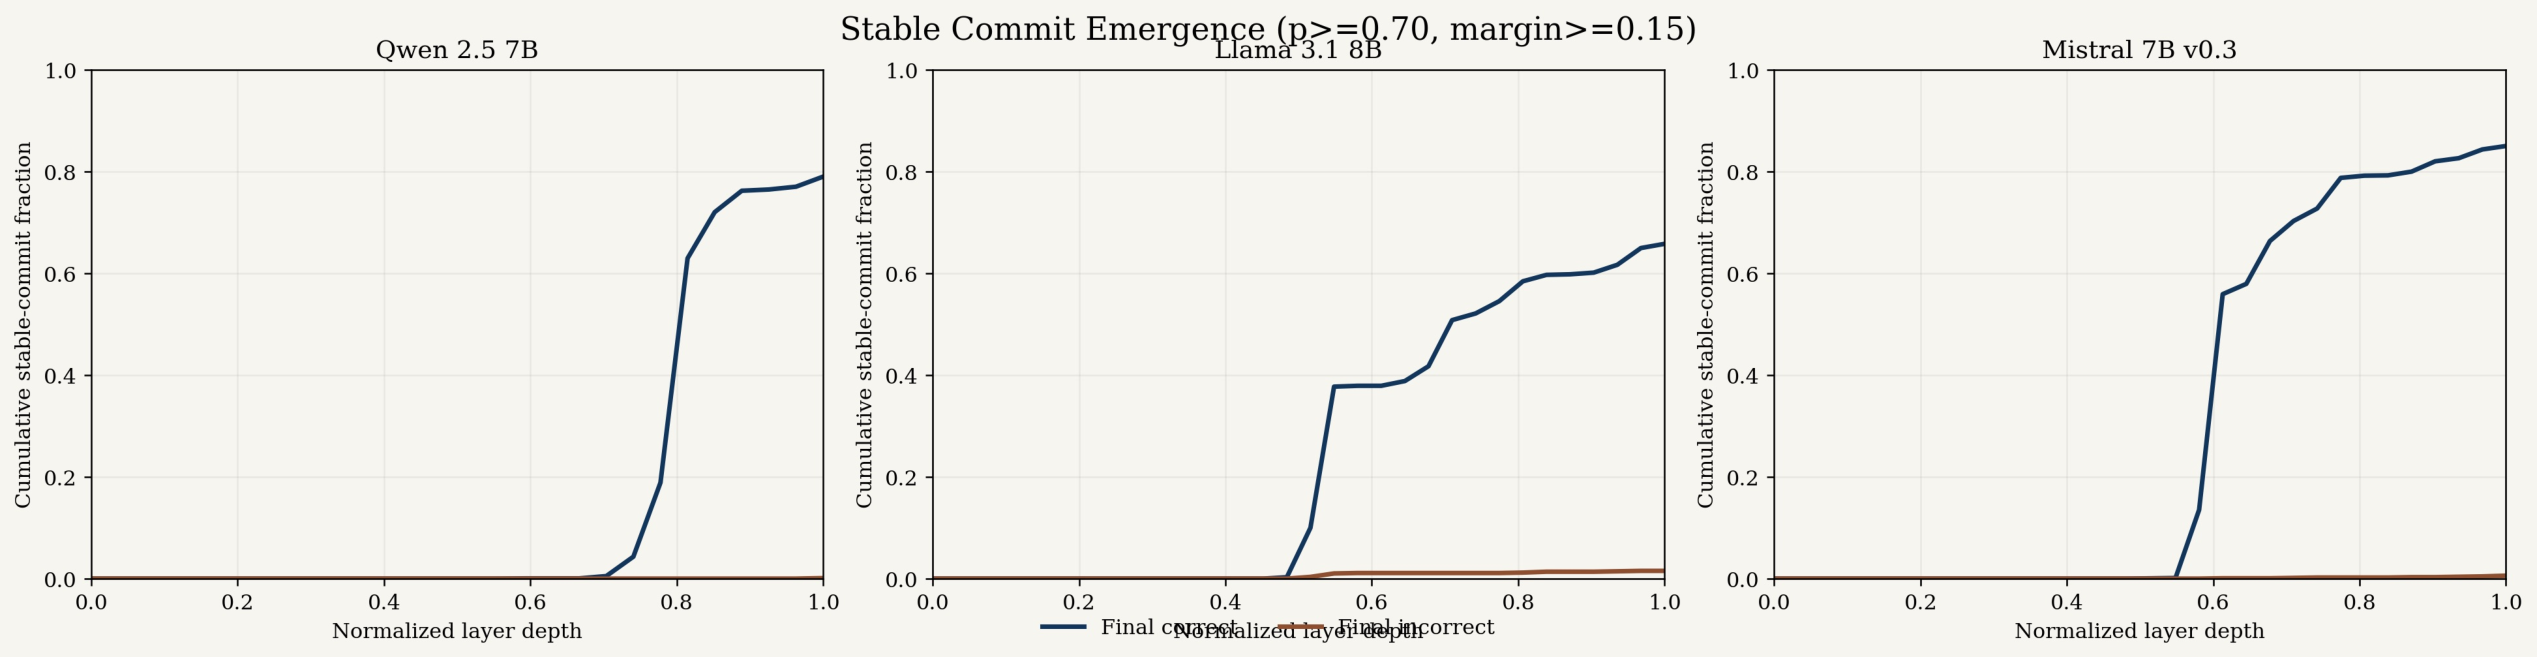
\includegraphics[width=\textwidth]{figures/commitment_cumulative_curves.pdf}
\caption{Cumulative distribution of commitment layers for converged prompts, stratified by final correctness. Vertical lines mark median commitment points.}
\label{fig:commitment}
\end{figure}

Figure~\ref{fig:commitment} shows cumulative commitment curves. Correct answers tended to commit earlier than incorrect ones across all models. Qwen exhibited the sharpest early commitment---over 50\% of correct answers committed by layer 15 (mid-network). Llama showed more gradual commitment with later median points.

\begin{figure}[ht]
\centering
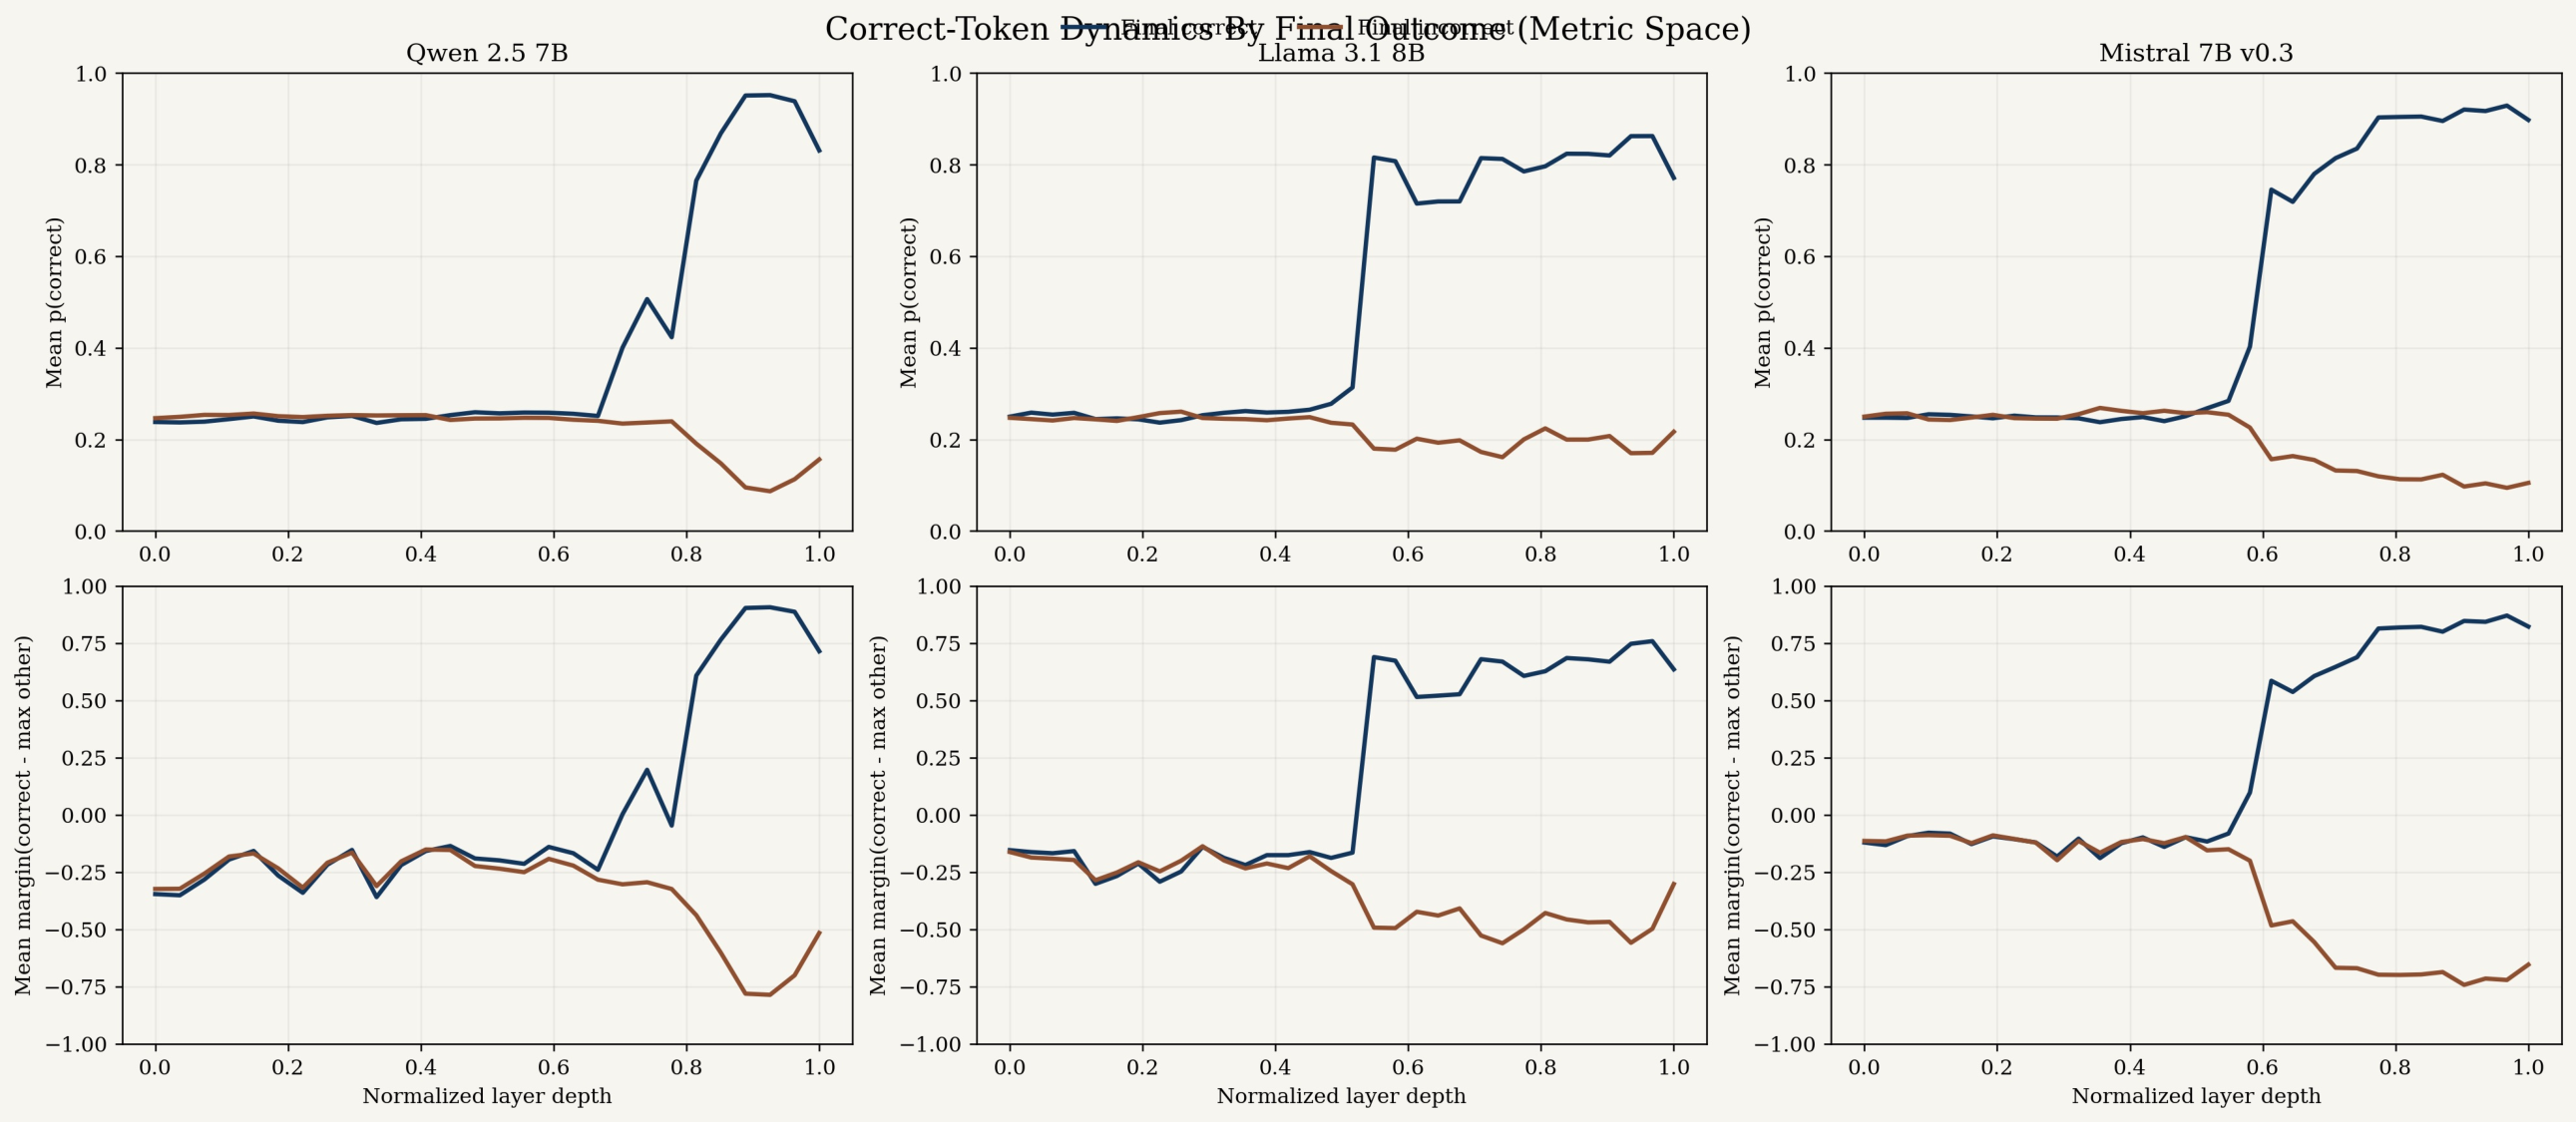
\includegraphics[width=0.8\textwidth]{figures/correct_token_dynamics_by_outcome.pdf}
\caption{Correct-token probability trajectories by final outcome. Shaded regions show standard error. Converged-correct trajectories rise steeply; non-converged trajectories remain flat or oscillate.}
\label{fig:trajectories}
\end{figure}

Figure~\ref{fig:trajectories} reveals distinct trajectory patterns. Converged-correct prompts showed monotonic probability increase from early layers. Non-converged prompts maintained flat or oscillating probabilities, suggesting models ``knew'' they were uncertain. This supports the hypothesis that models exhibit genuine confidence signals rather than overconfident guessing.

\subsection{Cross-Model Analysis: Universally Hard Prompts}

\begin{table}[ht]
\centering
\caption{Cross-model non-convergence overlap. Rows show prompts non-converged in $N$ models.}
\label{tab:crossmodel}
\begin{tabular}{cc}
\toprule
\textbf{Models Failed} & \textbf{Prompt Count} \\
\midrule
3 (all models) & 904 \\
$\geq$ 2 models & 1,491 \\
\bottomrule
\end{tabular}
\end{table}

A striking finding: 904 prompts (30.1\%) were non-converged in \textit{all three} models (Table~\ref{tab:crossmodel}). These ``universally hard'' prompts represent fundamental reasoning challenges---not architectural quirks but genuine knowledge or reasoning gaps.

\begin{figure}[ht]
\centering
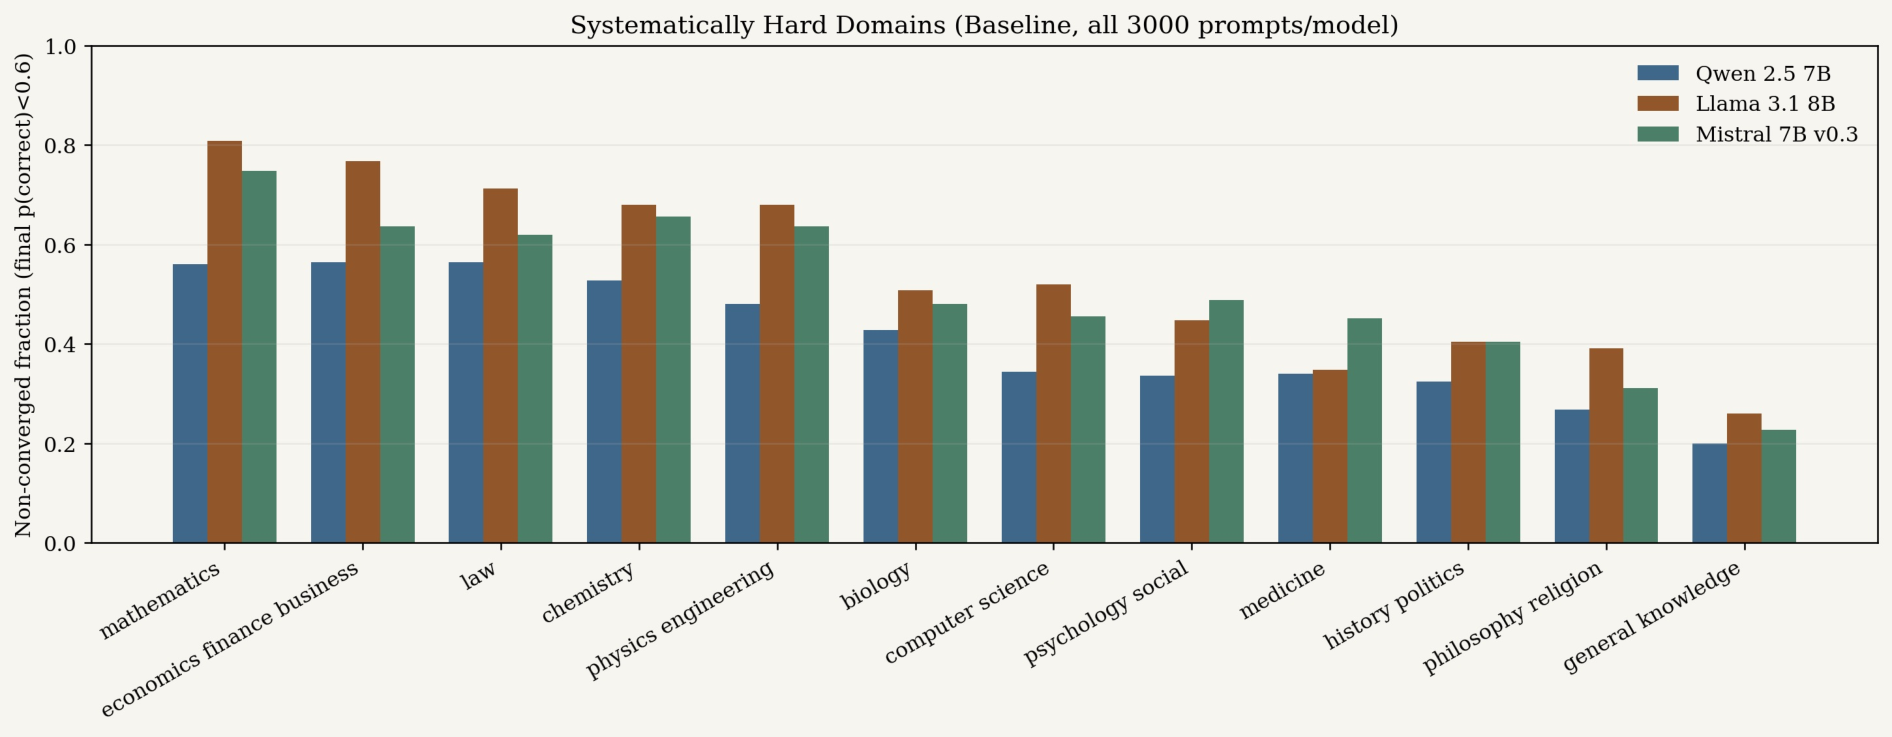
\includegraphics[width=0.8\textwidth]{figures/hard_domain_nonconvergence_rates.pdf}
\caption{Non-convergence rates by domain. Mathematics and economics/finance show highest difficulty; psychology/social and computer science show lowest.}
\label{fig:domains}
\end{figure}

Domain analysis (Figure~\ref{fig:domains}) revealed mathematics (70.5\%), economics/finance/business (65.6\%), and law (63.2\%) as hardest domains. Biology (47.2\%) and psychology/social (42.4\%) were relatively easier. This domain structure was consistent across models, further supporting the existence of fundamental difficulty factors.

\subsection{Early-Layer Predictability}

\begin{table}[ht]
\centering
\caption{Early-layer failure prediction performance.}
\label{tab:prediction}
\begin{tabular}{lcc}
\toprule
\textbf{Model} & \textbf{ROC-AUC} & \textbf{Average Precision} \\
\midrule
Qwen & 0.649 & 0.566 \\
Llama & 0.708 & 0.755 \\
Mistral & 0.704 & 0.705 \\
\bottomrule
\end{tabular}
\end{table}

Early-layer features predicted final non-convergence with ROC-AUC 0.65--0.71 (Table~\ref{tab:prediction}). Top predictive features included:

\begin{itemize}
    \item Numeric option count (positive coefficient: numeric options increase failure odds)
    \item Early $p(\text{correct})$ in lower quartile
    \item High option-pairwise Jaccard similarity (confusingly similar options)
    \item High early entropy / low early margin
\end{itemize}

\begin{figure}[ht]
\centering
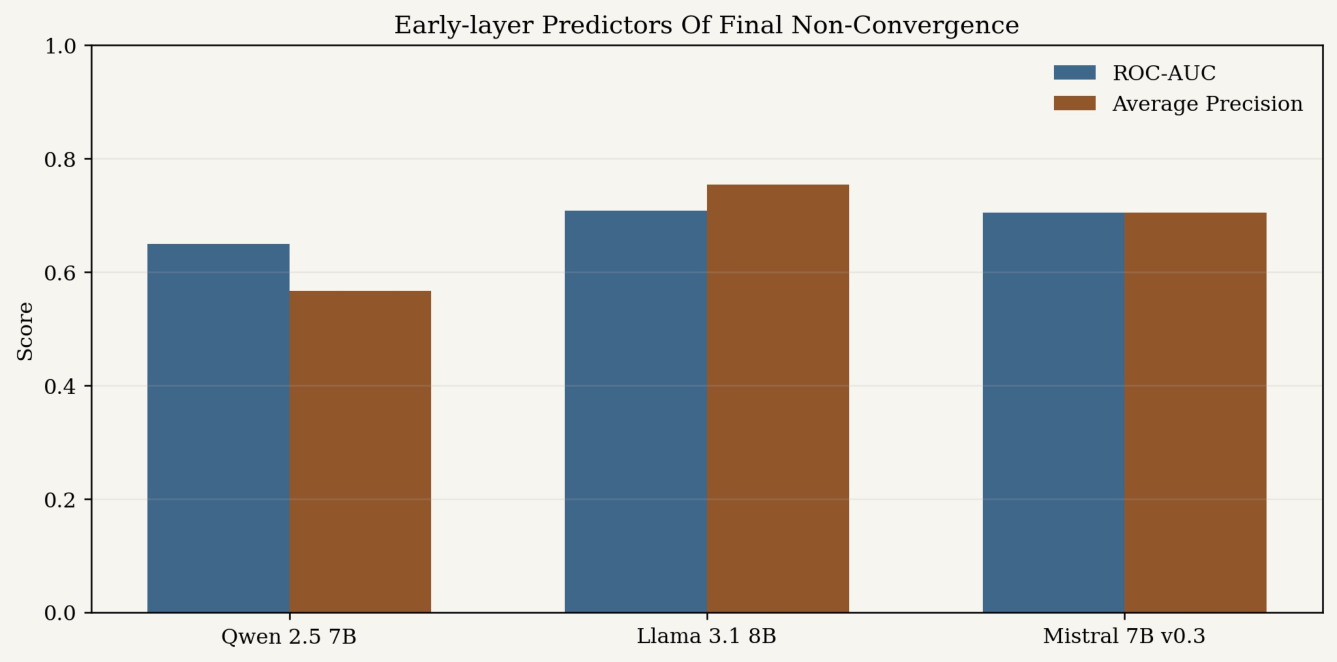
\includegraphics[width=0.6\textwidth]{figures/early_predictor_performance.pdf}
\caption{ROC curves for early-layer failure prediction. All models show significant predictability above chance (dashed line).}
\label{fig:roc}
\end{figure}

This predictability is remarkable: models ``know'' they will fail within the first 5--6 layers, evidenced by characteristic uncertainty patterns. This suggests potential for early-exit mechanisms or query reframing.

\subsection{Failure Mode Decomposition}

We decomposed non-converged prompts into failure mechanisms:

\begin{itemize}
    \item \textbf{Wrong direction}: Model drifts toward wrong answer (61.5--77.0\%)
    \item \textbf{Late instability}: Correct answer reached but abandoned (21.8--35.7\%)
    \item \textbf{Insufficient drift}: Model never strongly prefers any answer (0.2--1.2\%)
\end{itemize}

\begin{figure}[ht]
\centering
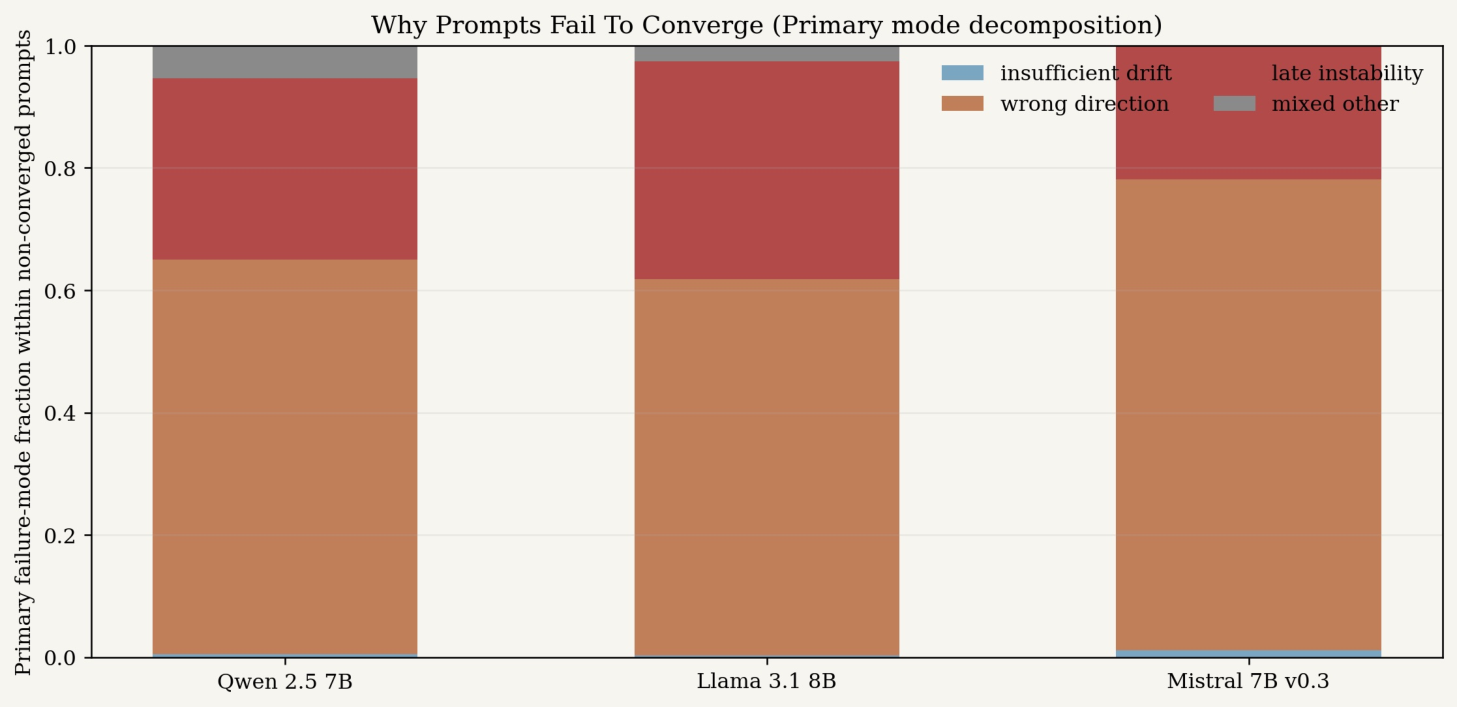
\includegraphics[width=0.8\textwidth]{figures/failure_mode_primary_breakdown.pdf}
\caption{Primary failure mode breakdown. ``Wrong direction'' dominates across all models.}
\label{fig:failures}
\end{figure}

Wrong-direction drift dominated (Figure~\ref{fig:failures}), indicating models often confidently commit to incorrect answers rather than remaining uncertain. Late instability was second-most common, especially for Llama (35.7\%), suggesting vulnerability to layer-wise perturbations.

\subsection{Representational Topology}

\begin{figure}[ht]
\centering
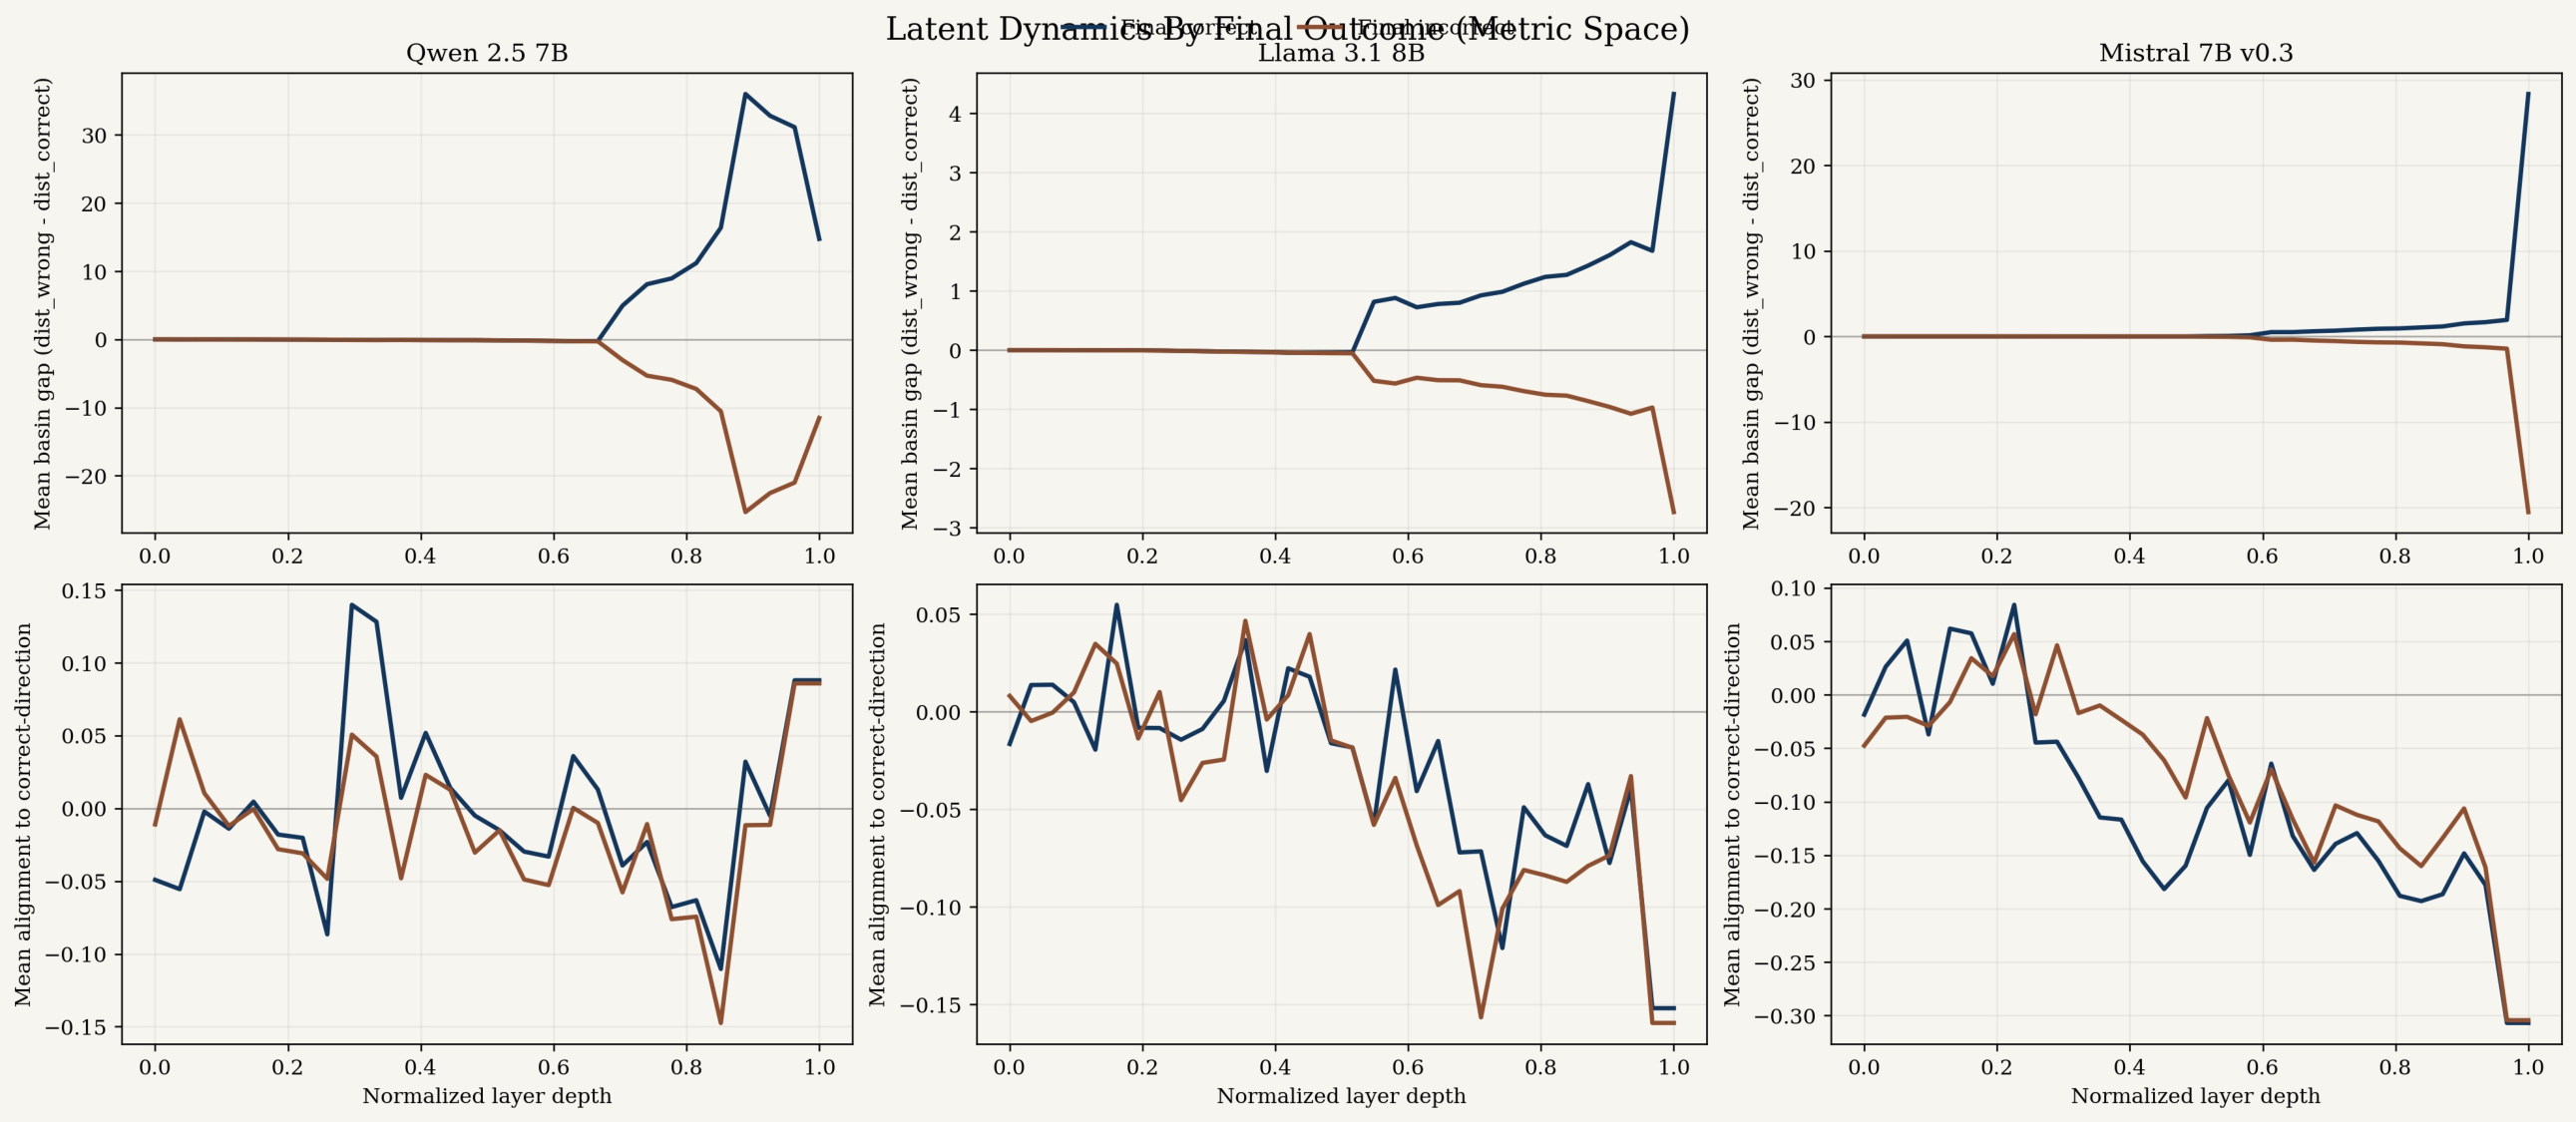
\includegraphics[width=0.8\textwidth]{figures/latent_dynamics_by_outcome.pdf}
\caption{Latent space dynamics: path length, trajectory alignment, and basin gap by outcome. Converged-correct prompts show higher alignment and basin separation.}
\label{fig:latent}
\end{figure}

Latent space analysis (Figure~\ref{fig:latent}) revealed:

\begin{itemize}
    \item \textbf{Path length}: Converged and non-converged prompts showed similar total path lengths, ruling out ``wandering'' as a failure mode
    \item \textbf{Trajectory alignment}: Converged-correct prompts exhibited stronger alignment between local steps and global direction
    \item \textbf{Basin gap}: Converged prompts showed larger separation from wrong-answer centroids
\end{itemize}

\begin{figure}[ht]
\centering
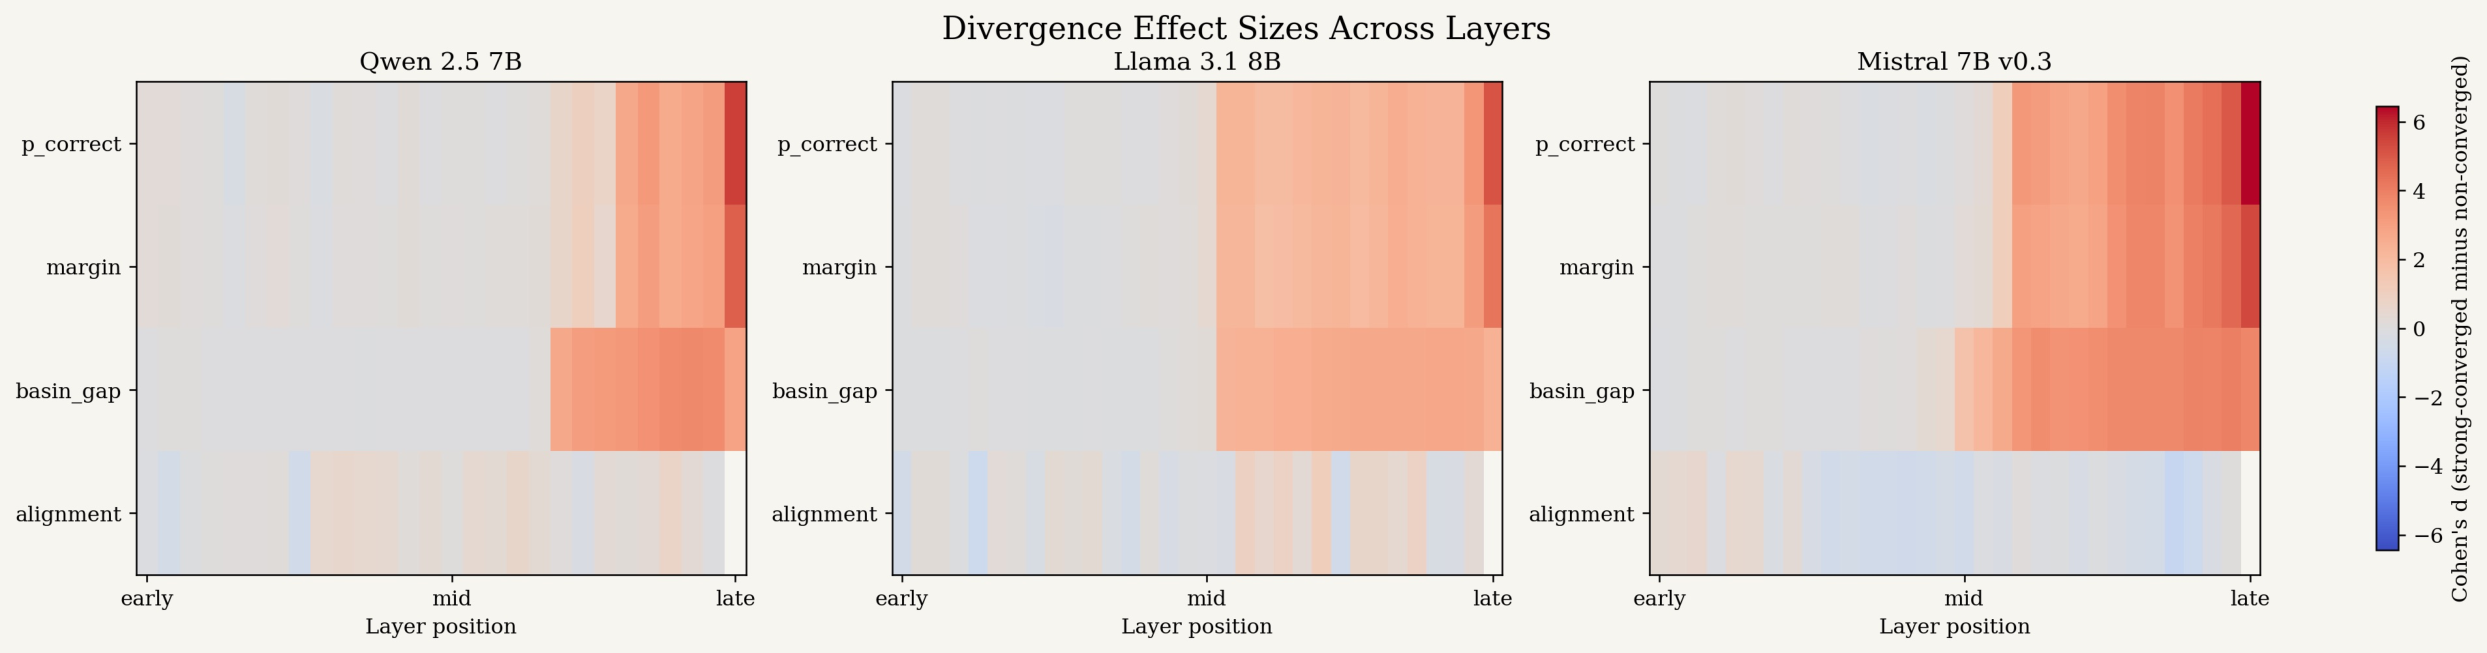
\includegraphics[width=0.8\textwidth]{figures/divergence_effect_heatmap.pdf}
\caption{Layer-window divergence effects between converged and non-converged trajectories. Darker cells indicate larger differences.}
\label{fig:divergence}
\end{figure}

Divergence analysis (Figure~\ref{fig:divergence}) identified critical layer windows where trajectories separated most:

\begin{itemize}
    \item Qwen: Layers 7--10 (alignment), 23--26 (basin gap), 24--27 (margin)
    \item Llama: Layers 18--22 (alignment), 26--30 (basin gap), 27--31 (margin)
    \item Mistral: Layers 9--13 (alignment), 27--31 (basin gap), 27--31 (margin)
\end{itemize}

These windows suggest targeted intervention points for activation steering or fine-tuning.

\section{Discussion}

\subsection{Implications}

Our findings carry several implications for LLM research and deployment:

\textbf{Structured decision formation exists.} Models do not merely sample from a static distribution; they exhibit progressive commitment with characteristic dynamics. This validates mechanistic interpretability approaches seeking to understand internal ``reasoning.''

\textbf{Early uncertainty predicts failure.} The predictability of non-convergence from early layers (ROC-AUC 0.65--0.71) suggests models possess ``metacognitive'' signals of their own uncertainty. This enables:
\begin{itemize}
    \item Early-exit mechanisms for efficiency
    \item Confidence calibration for reliability
    \item Query reframing for improved performance
\end{itemize}

\textbf{Universally hard prompts reveal fundamental gaps.} The 904 prompts challenging all models likely indicate reasoning patterns not well-captured by current training objectives. These warrant systematic study as ``reasoning stress tests.''

\textbf{Domain structure is consistent.} The consistent domain difficulty rankings across architectures suggests some domains genuinely require more complex reasoning, not just different knowledge distributions.

\subsection{Limitations}

This study has important limitations:

\textbf{Baseline-only scope.} Robustness analysis under prompt perturbations was deferred to future work. Claims about generalization across prompt variations are not supported.

\textbf{Multiple-choice constraint.} Our analysis is limited to forced-choice questions with objectively correct answers. Open-ended reasoning may exhibit different dynamics.

\textbf{Single-token focus.} We analyze first-step dynamics, which capture initial commitment but not multi-step reasoning chains.

\textbf{PCA subspace.} Topological analysis uses 128-dimensional projections, which may lose fine-grained geometric structure present in full hidden states.

\textbf{Model scale.} Results are limited to 7--8B parameter models. Larger models may exhibit different commitment dynamics.

\subsection{Related Work}

Our work connects to several research threads:

\textbf{Mechanistic interpretability.} Prior work has identified ``knowledge neurons'' \citep{dai2021knowledge}, ``induction heads'' \citep{elhage2021mathematical}, and ``logit lens'' techniques \citep{nostalgebraist2020logit} for analyzing internal representations. Our convergence framework extends these to decision dynamics.

\textbf{Confidence and calibration.} Studies of model calibration \citep{jiang2021can,desai2020calibration} have focused on output probabilities. We show internal layer-wise signals precede and predict final confidence.

\textbf{Failure prediction.} Prior work predicted model failures using various signals \citep{kadavath2022language}. We demonstrate prediction from early-layer internal features alone.

\textbf{Hard examples.} The identification of ``universally hard'' examples relates to work on adversarial examples \citep{wallace2019universal} and prediction difficulty 
\citep{swayamdipta2020dataset}.

\section{Conclusion}

This work introduces a framework for analyzing the ``shape of wisdom''---the geometry and dynamics of decision formation in large language models. Across three major open-weight models, we demonstrate:

\begin{enumerate}
    \item \textbf{Structured commitment}: Models exhibit progressive convergence with characteristic timing patterns
    \item \textbf{Predictable failures}: Early-layer features predict non-convergence (ROC-AUC 0.65--0.71)
    \item \textbf{Universal hardness}: 904 prompts resist convergence across all models, suggesting fundamental reasoning gaps
    \item \textbf{Topological structure}: Representational geometry reveals domain clustering and wrong-answer basins
\end{enumerate}

These findings establish that LLM decision-making is not an opaque sampling process but exhibits measurable structure amenable to analysis and intervention. Future work should extend this framework to robustness analysis, larger models, and open-ended reasoning domains.

\section*{Acknowledgments}

We thank the open-source community for releasing the models and datasets that enabled this research. Compute resources were provided by RunPod cloud GPU instances.

\bibliography{references}

\appendix

\section{Convergence Metric Definitions}

\begin{table}[ht]
\centering
\caption{Formal definitions of convergence metrics.}
\label{tab:definitions}
\begin{tabular}{lp{8cm}}
\toprule
\textbf{Metric} & \textbf{Definition} \\
\midrule
$p_{\text{correct}}(l)$ & Probability assigned to correct option at layer $l$ \\
$m_{\text{correct}}(l)$ & $p_{\text{correct}}(l) - \max_{k \neq c} p_k(l)$ \\
Strong convergence & $p_{\text{correct}}(L-1) \geq 0.8$ \\
Margin convergence & $m_{\text{correct}}(L-1) \geq 0.15$ \\
Stable commitment & Earliest layer where $p \geq 0.70$ and $m \geq 0.15$ for all subsequent layers \\
Late flip & Winner flip occurring in final 20\% of layers \\
\bottomrule
\end{tabular}
\end{table}

\section{Dataset Domain Distribution}

\begin{table}[ht]
\centering
\caption{Prompt counts by domain.}
\label{tab:domains}
\begin{tabular}{lc}
\toprule
\textbf{Domain} & \textbf{Count} \\
\midrule
Biology & 424 \\
Chemistry & 288 \\
Computer Science & 334 \\
Economics/Finance/Business & 291 \\
Law & 276 \\
Mathematics & 498 \\
Physics/Engineering & 506 \\
Psychology/Social & 383 \\
\midrule
\textbf{Total} & \textbf{3,000} \\
\bottomrule
\end{tabular}
\end{table}

\section{Model Architecture Details}

\begin{table}[ht]
\centering
\caption{Model specifications.}
\label{tab:models}
\begin{tabular}{lccc}
\toprule
\textbf{Model} & \textbf{Params} & \textbf{Layers} & \textbf{Hidden Dim} \\
\midrule
Qwen2.5-7B & 7.6B & 28 & 3,584 \\
Llama-3.1-8B & 8.0B & 32 & 4,096 \\
Mistral-7B-v0.3 & 7.3B & 32 & 4,096 \\
\bottomrule
\end{tabular}
\end{table}

\end{document}
